\documentclass[tikz]{standalone}
\usepackage{pgfplots}
\pgfplotsset{compat=1.15}
\usepackage{mathrsfs}
\usetikzlibrary{arrows,calc}
\usepackage{tkz-euclide}
\pagestyle{empty}

\definecolor{AngleClr}{rgb}{0,0.39215686274509803,0}
\definecolor{ShapeClr}{rgb}{0.6,0.2,0}
\definecolor{RedClr}{HTML}{b33229}

\begin{document}

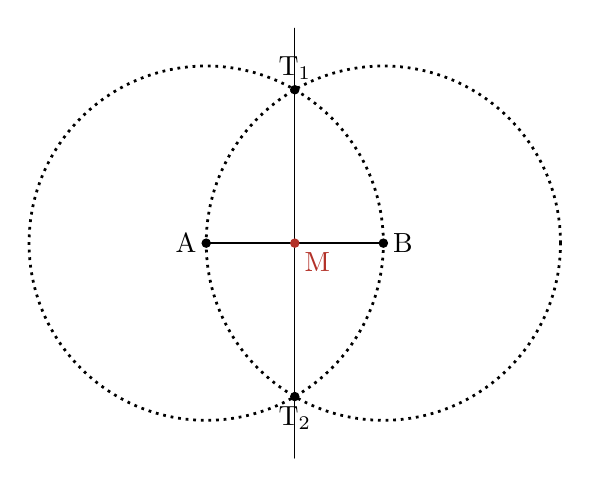
\begin{tikzpicture}[scale=.75]
\tkzSetUpLine[line width=1pt,color=black]
\tkzSetUpPoint[fill=black]

\tkzDefPoints{0/0/A,3/0/B}

\tkzDefMidPoint(A,B) \tkzGetPoint{M}

\tkzDrawCircles[line width=1.0pt, color=black,dashed,dash pattern=on 1pt off 1.75pt](A,B B,A)

\tkzInterCC(A,B)(B,A) \tkzGetPoints{T1}{T2}

\tkzDrawSegment[line width=0.5pt,color=black](A,B)
\tkzDrawSegment[line width=0.5pt,color=black, add=0.2 and 0.2](T1,T2)

\tkzDrawPoints[size=3](A,B,T1,T2)
\tkzDrawPoints[RedClr,size=3](M)

\tkzLabelPoint[left](A){$\rm A$}
\tkzLabelPoint[right](B){$\rm B$}
\tkzLabelPoint[above](T1){$\rm T_1$}
\tkzLabelPoint[below](T2){$\rm T_2$}
\tkzLabelPoint[RedClr,below right](M){$\rm M$}

\end{tikzpicture}

\end{document}
